\documentclass[]{article}

\usepackage{mathtools}
\usepackage{amssymb}
\usepackage{euler}
\usepackage{graphicx}
%opening
\title{Mathematik für Informatiker 3 - Serie 3}
\author{Tobias Reincke \\ Matrikelnummer 218203884}

\begin{document}

\maketitle


\section*{Aufgabe 1}
$(a_1 , a_2 ) \oplus (b_1 , b_2 ) := (a_1 + b_1 , a_2 + b_2 ) \\
(a_1 , a_2 ) \odot (b_1,b_2):= (a_1 b_1 , a_1 b_2 + a_2 b_1)$\\
$M :=\{(x,y) | x,y \in \mathbb{Q}\}$\\
Nach Definition ist (M , $\oplus$ , $\odot$) ein kommutativer Ring gdw. \\

\begin{itemize}
  \item{i)} (M, $\oplus$) eine abelsche Gruppe.
  
  \item{ii)} (M, $\odot$ ) eine abelsche Halbgruppe
  \item{iii)} Distributivitätgesetz gilt.
\end{itemize}



\subsection*{i)}
Assoziativitätsgesetz:\\
$ ( (a_1 , a_2 ) \oplus (b_1 , b_2 ) )  \oplus (c_1 , c_2 )   \\= (a_1 + b_1 , a_2 + b_2)\oplus (c_1 ,c _2 ) \\=(a_1 + b_1 +c_1, a_2 + b_2+c_1) \\= (a_1, a_2) \oplus (b_1 + c_1 , b_2 + c_2)\\ = (a_1, a_2) \oplus ( (b_1, b_2) \oplus (c_1, c_2) )   $ \\ \\
Das neutrale Element in (M, $\oplus$) ist (0,0). Es ist auch das einzige, da es die einzige Ergebnis folgender Gleichungen ist: \\
 $a_{1} = a_{1}+x_{1} \rightarrow x_1 = 0$\\
  $a_{2} = a_{2}+x_{2} \rightarrow x_2 = 0$\\
   Jedes Element $(a,b)$ ist invertierbar mit $(-a,-b)$ da: $(a+ (-a), b +(-b) ) = (0,0)$
   $\rightarrow$ (M, $\oplus$) ist Gruppe.
   (M, $\oplus$) ist abelsch: \\
   $(a_1 , a_2 ) \oplus (b_1 , b_2 ) = (a_1 + b_1 , a_2 + b_2 )= (b_1 + a_1 , b_2 + a_2 ) = (b_1 , b_2 ) \oplus (a_1 , a_2 ) $\\ 
   \textit{Das geht eigentlich aus der Assoziativität hervor. }
   
\subsection*{ii)}
Assoziativitätsgesetz:\\ \
  $  ((a_1 , a_2 ) \odot (b_1,b_2))\odot (c_1,c_2)\\= (a_1 b_1 , a_1 b_2 + a_2 b_1) \odot (c_1,c_2)\\
 =  (a_1 b_1c_1 , a_1b_1c_2+(a_1 b_2 + a_2 b_1)c_1 )\\ =(a_1 b_1c_1 , a_1b_1c_2+a_1 b_2 c_1 + a_2 b_1c_1 )\\
 =(a_1 b_1c_1 , a_1(b_1c_2+ b_2 c_1) + a_2 (b_1c_1) )\\  
  \textit{Das Erste mal das Zweite plus das Zweite mal das Erste}\\
 = (a_1,a_2) \odot (b_1c_1, b_1c_2+ b_2 c_1 ) \\
 =(a_1 , a_2 ) \odot ((b_1,b_2)\odot (c_1,c_2))$ \\
 Bewiesen! \\
 $a_1 * b_1 = a_1 \rightarrow b_1=1  \\
   a_2= 1*a_2 + b_2*a_1  \rightarrow 0= b_2*a_1 \rightarrow b_2=0  \\  \\$ Es gibt genau ein Neutrales Element 
   
   $ n = (1,0)!\\ $  n ist invertierbar mit sich selbst! $(M, \odot)$ ist Halbgruppe. \\
   $(M, \odot)$ ist abelsch. \\
   $(a_1 , a_2 ) \odot (b_1,b_2) \\= (a_1 b_1 , a_1 b_2 + a_2 b_1)\\ =(a_1 b_1 ,a_2 b_1+a_1 b_2 )\\ =(b_1,b_2 ) \odot (a_1,a_2) $
   
   \subsection*{iii)}
   Distributivgesetz: \\
   \textit{linkes:} \\
 $ (a_1,a_2) \oplus ( (b_1,b_2) \odot (c_1,c_2) ) =  ((a_1,a_2) \oplus  (b_1,b_2)  ) \odot ( (a_1,_2) \oplus  (c_1,c_2) )\\
 \rightarrow(a_1,a_2) \oplus (b_1c_1 , c_1b_2 + c_2b_1 ) = (a_1+b_1,a_2+b_2) \odot (a_1+c_1,a_2+c_2) \\ 
 \rightarrow  (a_1+b_1c_1 , a_2 +  c_1b_2 + c_2b_1) = (a_1a_1+ a_1b_1+a_1c_1, )
 \\ \\ \\ \\$
 
 
 
 
 
 
 
 
 
 
 
 
 
 
 
 
 
 
 
 
 
 
 $hi\\$
 $ (a_1,a_2) \odot ( (b_1,b_2) \oplus (c_1,c_2) ) =  ((a_1,a_2) \odot  (b_1,b_2)  ) \oplus ( (a_1,_2) \odot(c_1,c_2) )\\
\rightarrow (a_1,a_2) \odot (b_1+c_1,b_2+c_2) = (a_1b_1, )
 $
                                

\section*{Aufgabe 2}
\section*{Aufgabe 3}
\section*{Aufgabe 4}
RSA-Algorithmus:\\
geg: Primzahlen $p:=11, q :=17$ ;  private Key $g :=97 ; n = 11*17$ vom Empfänger \\ g ist teilerfremd zu 160, g ist sogar prim! \\
$m:= \phi(n) = (p-1)(q-1)= 10*16=160 $
Ermitteln von k : 33 (via Code)\\
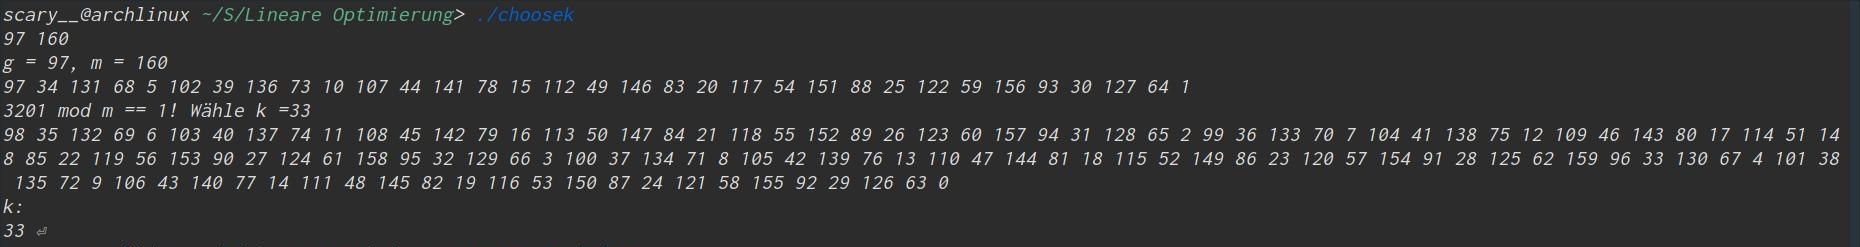
\includegraphics[width=\textwidth,clip,trim=0 0 {500} 0, ]{k.jpg} \\
\\
Senden von $k=33$ und $n= 187$ an Absender (öffentlich)\\
geg: $a:=20$
Absender verschlüsselt:  $e:= a^k \mod=20^{33}\mod 160=8589934592000000000000000000000000000000000 \mod 160=0 $\\
Zur Herleitung: $20^{33} \mod 160 = 2^{33}*2^{33}*5^{33} \mod 2*2*2*2*2*5=2^{66}*5^{33}\mod 2^5*5 = 0$ \\
Absender verschickt Zahl $e=0$
Empfänger entschlüsselt $b:= e^g \mod \ n = 0^{97} \mod 187 = 0  $\\  Dabei gilt: \\
$a = b \leftrightarrow 0=20  $  Irgendwas ist hier falsch..  

	\begin{figure}[!h]
\centering
	\includegraphics[width=0.7\linewidth]{"prove.jpg"}
	
	\label{fig:screenshot-from-2019-11-30-17-46-06}
	
\end{figure}


\section*{Aufgabe 5}


\end{document}